\section{Технический проект}

\subsection{Архитектура и взаимодействие компонентов программной системы}

Разработанная информационная система представляет собой конфигурацию для платформы «1С:Предприятие 8.3», функционирующую в режиме файловой информационной базы. Архитектура решения соответствует классической модели, заложенной в платформу: данные хранятся в объектах конфигурации (справочниках, документах, регистрах), бизнес-логика сосредоточена в программных модулях, а пользовательский интерфейс реализован в виде управляемого приложения.

Центральным принципом работы системы является событийная модель. Все значимые операции (составление расписания, проведение соревнований, движение инвентаря) оформляются в виде документов. В момент проведения документа платформа автоматически формирует записи в регистрах, обеспечивая тем самым целостность, непротиворечивость и хронологическую упорядоченность данных. Такой подход позволяет в любой момент времени получить актуальный срез информации, будь то расписание на конкретную дату или текущий остаток спортивного инвентаря.

Архитектура системы построена по трехуровневому принципу, соответствующему стандартам платформы 1С:Предприятие 8.3. Верхний уровень представления обеспечивает взаимодействие пользователей с системой через управляемый интерфейс. Средний уровень бизнес-логики содержит программные модули, реализующие обработку данных. Нижний уровень данных включает справочники, документы и регистры, хранящиеся в файловой базе данных. Файловый режим работы выбран в связи с небольшим количеством одновременно работающих пользователей, что позволило избежать необходимости развертывания выделенного сервера СУБД. Общая схема взаимодействия компонентов системы в рамках данной архитектуры представлена на рисунке 3.1.

\begin{center}
	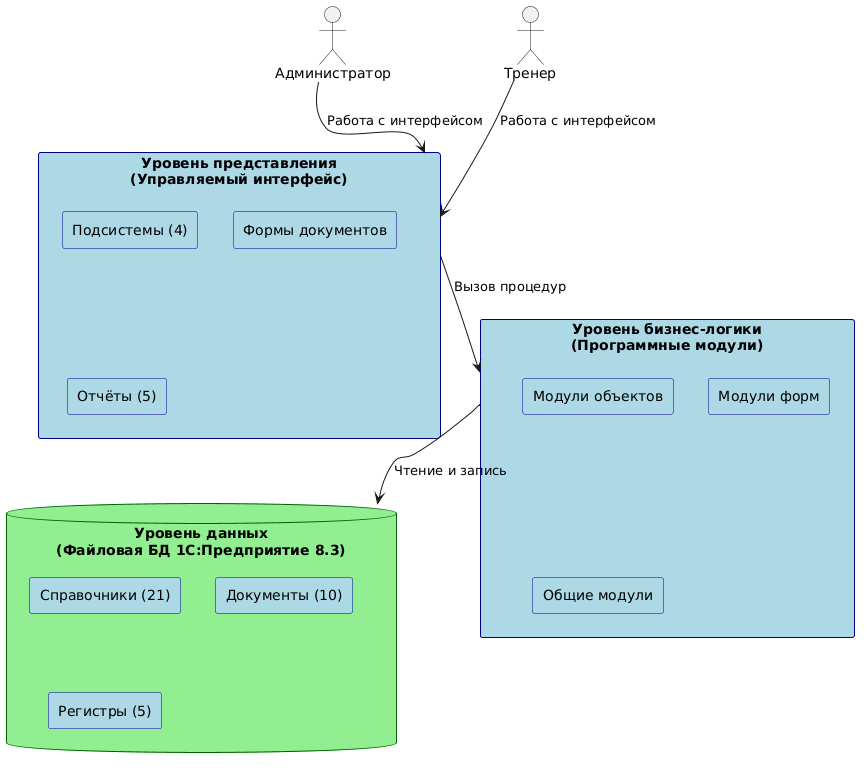
\includegraphics[width=0.9\textwidth]{images/ris3_1.png}
\end{center}
\begin{center}
{Рисунок 3.1 - Общая схема взаимодействия компонентов системы}
\end{center}

\subsection{Обоснование выбора платформы проектирования}

Платформа «1С:Предприятие 8.3» была выбрана в качестве среды разработки из-за совокупности факторов, позволяющие успешно выполнить проект.

Платформа предоставляет интегрированную среду быстрой разработки, включающую визуальные конструкторы форм, справочников и документов. Это позволило в сжатые сроки создать полнофункциональное приложение, не прибегая к программированию рутинных операций по созданию пользовательского интерфейса. Там, где требовалась нестандартная логика, использовался встроенный язык программирования, не уступающий современным процедурным языкам.

Наличие встроенной системы компоновки данных (СКД) дало возможность создавать аналитические отчеты различной сложности декларативно, без написания программного кода. Гибкая ролевая модель позволила реализовать разграничение прав доступа, критически важное для информационных систем с несколькими категориями пользователей. Наконец, возможность работы в файловом режиме избавила от необходимости развертывания и администрирования выделенного сервера СУБД, что особенно актуально для небольших организаций, таких как спортивные школы.

В качестве альтернатив рассматривались разработка с использованием веб-стека (языки Python, PHP, JavaScript) и различных СУБД, а также адаптация существующих коробочных решений. Однако эти варианты были отклонены по причинам значительно более высокой трудоемкости и стоимости разработки, а также ограниченной гибкости готовых продуктов.

\subsection{Структура конфигурации}

Информационная база системы включает в себя 21 справочник, 10 документов, 4 перечисления, 1 регистр накопления и 4 регистра сведений. Такая структура является типовой для прикладных решений на платформе 1С и обеспечивает четкое разделение данных на нормативно-справочную информацию (справочники), оперативные данные (документы) и агрегированные показатели (регистры).

Справочники образуют фундамент системы, храня информацию о спортсменах, тренерах, группах, видах спорта, помещениях и других сущностях. Документы, в свою очередь, фиксируют все изменения и события, происходящие в процессе работы школы. При проведении каждого документа формируются движения по регистрам, которые аккумулируют данные в разрезах, необходимых для последующего анализа и построения отчетов. Наглядное представление состава объектов конфигурации приведено на рисунке 3.2.

\begin{center}
	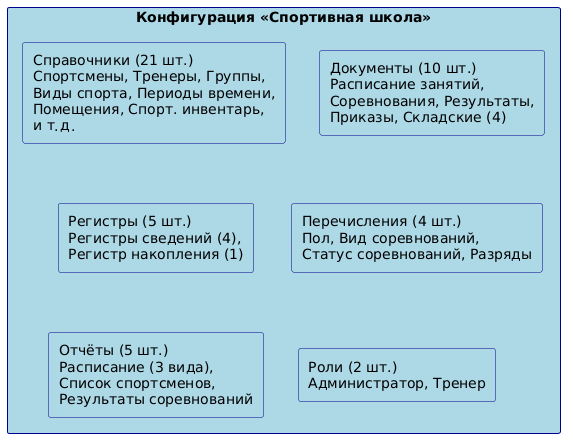
\includegraphics[width=0.9\textwidth]{images/ris3_2.png}
\end{center}
\begin{center}
{Рисунок 3.2 - Состав объектов конфигурации}
\end{center}

\subsection{Структура справочников}

Центральное место в системе занимает справочник «Спортсмены», аккумулирующий все сведения об учащихся. Помимо стандартных анкетных данных (ФИО, дата рождения, пол, контактная информация), он содержит табличную часть «Виды спорта», где для каждого спортсмена фиксируется вид спорта и присвоенный спортивный разряд. Это решение позволяет отразить ситуацию, когда один учащийся тренируется по нескольким видам и имеет по ним различные разряды.

Справочник «Тренеры» помимо анкетных данных содержит указание на специализацию (вид спорта) и должность. Это используется при составлении расписания для автоматической фильтрации тренеров по их профилю. Справочник «Группы» связывает учебные группы с конкретным видом спорта. Справочник «Периоды времени» задает временные слоты, из которых впоследствии формируется сетка расписания.

Ключевым классификатором является справочник «Виды спорта», выступающий владельцем для подчиненного ему справочника «Спортивные дисциплины». Такая связь позволяет для каждого вида спорта вести собственный уникальный перечень дисциплин.Это исключает смешение данных между разными видами спорта и упрощает фильтрацию при выборе дисциплины в документах «Соревнования» и «Результаты соревнований».

В таблице 3.1 приведен перечень основных справочников системы с указанием их назначения.

\vspace{0.5cm}
\noindent
{Таблица 3.1 - Основные справочники системы}

\vspace{0.2cm}
\noindent
\begin{tabular}{|p{5cm}|p{10.5cm}|}
	\hline
	{Справочник} & {Назначение} \\
	\hline
	Спортсмены & Хранение анкетных данных учащихся, видов спорта и разрядов \\
	\hline
	Тренеры & Хранение данных о тренерском составе, специализации \\
	\hline
	Группы & Перечень учебных групп с привязкой к виду спорта \\
	\hline
	Виды спорта & Классификатор видов спорта, владелец для дисциплин \\
	\hline
	Спортивные дисциплины & Перечень дисциплин, подчинен видам спорта \\
	\hline
	Периоды времени & Временные слоты для составления расписания \\
	\hline
	Помещения & Места проведения тренировок и соревнований \\
	\hline
	Спортивный инвентарь & Номенклатура инвентаря для складского учета \\
	\hline
	Спортивные разряды & Классификатор спортивных разрядов и званий \\
	\hline
	Поставщики & Организации, поставляющие спортивный инвентарь \\
	\hline
	Спортивные судьи & Данные о судейском составе \\
	\hline
	Статус соревнований & Классификатор уровней соревнований \\
	\hline
\end{tabular}

\newpage

Взаимосвязи между ключевыми сущностями системы представлены на рисунке 3.3.

\begin{center}
	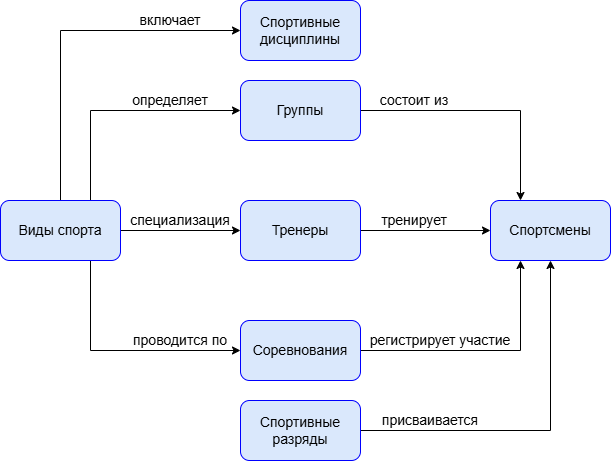
\includegraphics[width=0.9\textwidth]{images/er_diagramma2.png}
\end{center}
\begin{center}
{Рисунок 3.3 - Схема связи ключевых сущностей системы}
\end{center}

\subsection{Структура документов}

Основным операционным документом системы является «Расписание занятий», предназначенный для планирования тренировочного процесса на календарный месяц. Его табличная часть построена по принципу матрицы: строки определяют связку «тренер - группа - место проведения», а колонки соответствуют дням недели, в ячейках которых проставляются временные интервалы из справочника «Периоды времени». При проведении документ генерирует записи в регистрах сведений, делая расписание доступным для анализа в отчетах.

Документ «Соревнования» отличается сложной структурой, включающей три табличные части: «Дисциплины», «Участники» и «Судьи», что позволяет всесторонне описать спортивное мероприятие. На его основании вводится документ «Результаты соревнований», для которого реализована функция массовой загрузки данных из файлов Microsoft Excel, что значительно ускоряет работу при обработке большого количества результатов.

Цепочка оформления спортивных разрядов автоматизирована документами «Заявка на присвоение разрядов» и «Приказ о присвоении разряда». Последний имеет печатную форму, генерируемую по утвержденному шаблону.

Учет спортивного инвентаря реализован набором из четырех документов: «Поступление», «Выдача», «Возврат» и «Списание». Все они при проведении формируют движения по регистру накопления «Спортивный инвентарь организации».

В таблице 3.2 приведен полный перечень документов системы с указанием формируемых ими движений по регистрам.

\newpage

\noindent
{Таблица 3.2 - Документы системы и формируемые движения}
\par\vspace{0.2cm}
\noindent
\begin{tabular}{|p{6cm}|p{9.5cm}|}
		\hline
		{Документ} & {Формируемые движения (регистры)} \\
		\hline
		Расписание занятий & Регистры сведений «Расписание занятий», «Расписание занятий группы» \\
		\hline
		Приказ о назначении тренера & Регистр сведений «Тренер спортсмена» \\
		\hline
		Соревнования & Без движений (регистрация факта) \\
		\hline
		Результаты соревнований & Регистр сведений «Результаты соревнований» \\
		\hline
		Заявка на присвоение разрядов & Без движений (основание для приказа) \\
		\hline
		Приказ о присвоении разряда & Без движений (итоговый документ) \\
		\hline
		Поступление инвентаря & Регистр накопления «Спортивный инвентарь организации» (приход) \\
		\hline
		Выдача инвентаря & Регистр накопления «Спортивный инвентарь организации» (расход, приход на МОЛ) \\
		\hline
		Возврат инвентаря & Регистр накопления «Спортивный инвентарь организации» (приход, расход с МОЛ) \\
		\hline
		Списание инвентаря & Регистр накопления «Спортивный инвентарь организации» (расход) \\
		\hline
\end{tabular}
\vspace{0.4cm}

\subsection{Регистры}

Для накопления и хранения оперативных данных используются регистры двух типов.

Регистр накопления «Спортивный инвентарь организации» работает в режиме «Остатки» и позволяет в любой момент времени получить информацию о количестве каждой единицы инвентаря в разрезе материально-ответственных лиц (спортсменов или тренеров). Движения по регистру формируются автоматически при проведении складских документов.

Регистры сведений «Расписание занятий» и «Расписание занятий группы» являются хранилищем данных о расписании, заполняемым документом «Расписание занятий». На их основе строятся все отчеты по расписанию. Регистр «Тренер спортсмена» фиксирует историю назначений наставников, а регистр «Результаты соревнований» накапливает статистику выступлений. Использование периодических регистров сведений гарантирует сохранность всей истории изменений.

\subsection{Программная реализация}

Наиболее сложным в алгоритмическом плане является модуль формы документа «Расписание занятий». Для удобства заполнения расписания в документе используется табличная часть, где строки содержат тренера, группу и место проведения, а колонки соответствуют дням недели. В каждой ячейке пользователь выбирает временной интервал из справочника «Периоды времени». Проведение документа формирует записи в регистрах сведений, на основе которых в дальнейшем строятся отчеты.

Алгоритм программного заполнения планировщика относится к отчету «Расписание занятий общее», где данные уже не редактируются, а только отображаются. Для этого отчета используется элемент управления «Планировщик», заполнение которого выполняется полностью программно. Алгоритм построен на многоуровневом обходе иерархического результата запроса к регистру сведений. На первом уровне данные группируются по видам спорта, на втором - по тренерам, на третьем - по группам. Для каждого занятия вычисляются координаты на временной сетке планировщика, после чего создается визуальный элемент. Для улучшения восприятия различные уровни иерархии и сами занятия выделяются цветом. Внешний вид сформированного отчета представлен на рисунке 3.4.

Кроме того, программно реализована функция импорта данных в документ «Результаты соревнований» из файлов Excel. Процедура считывает табличный документ, выполняет сопоставление строк со справочниками спортсменов и дисциплин по наименованию и автоматически заполняет табличную часть документа.

\vspace{0.5cm}
\begin{center}
	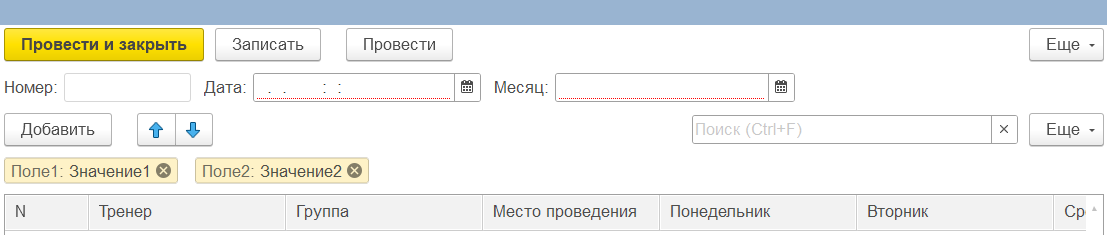
\includegraphics[width=1\textwidth, height=4.cm]{images/raspis_tabl.png}
\end{center}
\begin{center}
	{Рисунок 3.4 - Форма документа «Расписание занятий»}
\end{center}
\vspace{0.5cm}

\subsection{Пользовательский интерфейс}

Интерфейс системы реализован в полном соответствии с требованиями технического задания. Все четыре подсистемы, перечисленные в разделе 2.4, реализованы и функционируют. Каждая подсистема объединяет функционально связанные объекты, что делает навигацию интуитивно понятной и снижает время на поиск нужной команды.

Все формы документов и справочников выполнены в едином стиле управляемого приложения. Командные панели форм предоставляют пользователю как стандартные действия («Провести и закрыть», «Записать», «Провести»), так и дополнительные команды, специфичные для конкретных документов. Документ «Результаты соревнований» содержит кнопку «Заполнить из файла» для импорта данных из Excel, документ «Соревнования» - кнопку «Отправить напоминание по эл. почте», а документ «Приказ о присвоении разряда» - кнопку «Печать» для формирования официальной печатной формы.

Для визуализации расписания занятий применен специализированный элемент управления «Планировщик». По вертикальной оси планировщика располагается иерархический список с группировкой занятий по видам спорта, тренерам и группам. По горизонтальной оси отображается шкала дней месяца с детализацией по часам. Каждое занятие отображается в виде цветной плашки, что делает восприятие расписания наглядным и удобным для пользователя.

\subsection{Разграничение прав доступа}

Для обеспечения информационной безопасности и разграничения зон ответственности в системе реализованы две роли: «Администратор» и «Тренер». Разграничение прав выполнено штатными средствами платформы 1С:Предприятие через механизм ролей. Для каждой роли настроены индивидуальные права на чтение, просмотр, добавление, изменение и удаление по каждому объекту конфигурации.

Администратор обладает полным набором прав на все объекты конфигурации: может создавать, редактировать и удалять записи справочников, оформлять и проводить любые документы, формировать отчеты, управлять учетными записями пользователей и настраивать параметры электронной почты.

Тренер имеет доступ только к тем объектам, которые непосредственно связаны с его профессиональной деятельностью: просмотр расписания, справочников спортсменов и групп, просмотр информации о соревнованиях, внесение и редактирование результатов соревнований, учет спортивного инвентаря При этом для тренера полностью закрыт доступ к оформлению приказов и системным настройкам. При входе в систему платформа автоматически определяет роль пользователя и формирует интерфейс, отображая только те подсистемы и команды, которые разрешены данной роли.

\subsection{Обеспечение надежности и целостности данных}

Требования к надежности, сформулированные в техническом задании, реализованы в системе с использованием следующих механизмов.

Все операции, связанные с проведением документов, выполняются в рамках транзакций. В случае возникновения ошибки на любом этапе проведения документ все изменения автоматически откатываются, и документ остается в исходном состоянии.

Контроль уникальности номеров документов и кодов справочников реализован стандартными механизмами платформы. При попытке сохранить запись с уже существующим кодом или номером система автоматически блокирует операцию и выводит информативное сообщение.

Валидация входных данных выполняется на уровне платформы при проведении документов. Все обязательные реквизиты, отмеченные в конфигурации как подлежащие проверке, контролируются автоматически. При обнаружении незаполненных полей система выводит сообщение об ошибке и не позволяет провести документ до устранения недостатков.

Для обеспечения сохранности данных предусмотрено регулярное резервное копирование информационной базы штатными средствами платформы - выгрузка в формат .dt через конфигуратор. Данная операция позволяет сохранить как структуру конфигурации, так и все пользовательские данные в одном файле, который может быть загружен на другом компьютере для полного восстановления системы.

\subsection{Эксплуатация и развертывание}

Система функционирует в файловом режиме, что избавляет от необходимости развертывания и администрирования выделенного сервера СУБД. Для начала работы достаточно установить платформу «1С:Предприятие 8.3» (учебная версия) на компьютер под управлением операционной системы Windows 10 или Windows 11 и открыть файл информационной базы.

Для использования функции почтовых оповещений требуется наличие доступа к сети Интернет. Остальной функционал системы доступен полностью автономно, без подключения к внешним ресурсам.

Рекомендуемая минимальная конфигурация компьютера: процессор с тактовой частотой от 2 ГГц, оперативная память от 4 ГБ, свободное дисковое пространство от 10 ГБ. Данные характеристики соответствуют минимальным требованиям платформы «1С:Предприятие 8.3» и являются типовыми для большинства современных офисных компьютеров.

При необходимости масштабирования система может быть переведена в клиент-серверный режим с использованием СУБД PostgreSQL, что позволит увеличить количество одновременно работающих пользователей и повысить отказоустойчивость.